\chapter{Background}
\section{Cryptography}

Cryptography is the science of securing information through encryption. Encryption or ciphering refers to the process of making a message incomprehensible \cite[18]{crypto} The security of all cryptographic methods is essentially based on the difficulty of guessing a secret key or obtaining it by other means. It is possible to guess a key, even if the probability becomes very small as the length of the key increases. It must be pointed out that there is no absolute security in cryptography \cite[25]{crypto}.

Practically all cryptographic methods have the task of ensuring one of the following security properties are met \cite[18]{crypto}. 
\begin{itemize}
    \item \textbf{Confidentiality} The aim of confidentiality is to make it impossible or difficult for unathorized persons to read a message \cite[18]{crypto}.
    \item \textbf{Authenticity} Proof of identity of the message sender to the recipient, i.e. the recipient can be sure that the message does not originate from another (unauthorized) sender \cite[18]{crypto}
    \item \textbf{Integrity} The message must not be altered (by unauthorized persons) during transmission. It retains its integrity \cite[18]{crypto}.
    \item \textbf{Non-repudiation} The sender cannot later deny having sent a message \cite[18]{crypto}.
\end{itemize}

Cryptographic algorithms are mathematical equations, i.e. mathematical functions for encryption and decryption \cite[19]{crypto}. A cryptographic algorithm for encryption can be used in a variety of ways in different applications. To ensure that an application always runs in the same and correct correct way, cryptographic protocols are defined. In contrast to the cryptographic algorithms, the protocols are procedures for controlling the flow of transactions for certain applications. \cite[22]{crypto}.

\section{Cryptography in Voting Systems}
The idea of combining cryptographic methods with voting systems is not new. In 1981, David Chaum published a cryptographic technique based on public key cryptography that hides who a participant communicates with, aswell as the content of the communication. The untracable mail system requires messages to pass through a cascade of mixes (also known as a Mix Network) \cite[86]{chaum}. Chaum proposes that the techniques can be used in elections in which an individual can correspond with a record-keeping organisation or an interested party under a unique pseudonym. The unique pseudonym has to appear in a roster of accetable clients. A interested party or record keeping organisation can verify that the message was sent by a registered voter. The record-keeping organisation or the interested party can also verify that the message was not altered during transmission. \cite[84]{chaum}. 

In this use case, the properties of Confidentiality, Authenticity, Integrity and Non-repudiation are ensured. However, to be worthy of public trust, an election process must give voters and observers compelling evidence (e.g. verifiability) that the election was conducted properly without breaking ballot secrecy. The problem of public trust is further exacerbated to now having to trust election software and hardware, in addition to election officials, and proceedurs. Fortunetly, modern cryptography provides viable methods for achieving the properties of verifiability and ballot secrecy. \cite[6]{stuve-studys}. The goal of these methods is to place as little trust as possible in the individual components of the voting system, in order to be able to convince oneself as an independent auditor of the correctness of the final result, while at the same time not revealing more information about the individual votes than can be derived from the final result anyway. \cite[6, 10]{stuve-studys}.

According to a study published by the German Federal Office for Information Security (BSI), End-to-end verifiability is the gold standard to achieve these goals \cite[10]{stuve-studys}. Furthermore, the Voluntary Voting System Guidelines (VVSG) 2.0 adopted by the U.S. Election Assitance Commission (EAC) states that a voting system need to be software independent. The VVSG 2.0 currently states only two methods for achieving software independence. The first through the use of independent voter-verifiable paper records, and the second through cryptographic end-to-end verifiable voting systems. \cite[181]{vvsg}.The VVSG is intended for designers and manufacturers of voting systems.\cite{vvsg-intro}.

\section{End-to-End Verifiability}

End-to-end verifiability has two principal components \cite[2]{e2e-primer}:
\begin{itemize}
    \item \textbf{Cast As Intended} voters can verify that their selections (whether indicated electronically, on
    paper, or by other means) are correctly recorded, and \cite[2]{e2e-primer}.
    \item \textbf{Tallied As Cast} any member of the public can verify that every recorded vote is correctly
    included in the tally. \cite[2]{e2e-primer}.
\end{itemize}

All E2E Verifiable Voting Systems have cryptographic building blocks at their core. The most important recurring cryptographic building blocks are \cite[13]{stuve-studys}:

All verifiable voting systems have cryptographic building blocks at their core. The most important recurring cryptographic building blocks are:
\begin{itemize}
    \item Public-key encryption is used in most verifiable voting systems to encrypt sensitive data, such as votes, with a public key so that only selected parties who know the corresponding secret key can read it
    \item Commitments are often used for similar purposes, with the difference that the sensitive data cannot be read with a message-independent secret key, but only with specific information that is generated during the individual commit process and then shared with selected parties
    \item Digital signatures are commonly used in voting systems so that different parties 
    can verify that the messages they receive are from the indicated party.
    \item Zero-knowledge proofs allow a party to prove that it performed a certain computational step correctly, without having to reveal any further information (such as the secret key used in the computation). These building blocks are central to combine the competing but desirable properties of public verifiability and secrecy of votes.
    \item Threshold secret sharing can be used to distribute information about a secret (e.g., a secret key) among multiple parties, so that more than a certain threshold of them must cooperate to recover the secret from their individual shares.
\end{itemize}

\section{E2E Verifiable Software Libraries}
Implementing a E2E Verifiable Voting System is a complex task. It requires a person or a group of persons implementing the voting system to have skills cryptography in addition to a "standard" background of a software engineer. The person or group must understand the particular algorithm or to implement it correctly. Luckily, there are several high-quality and well-maintained software libraries that implement the cryptographic building blocks at the core of E2E Verifiable Voting Systems. For example, CHVote, ElectionGuard, Verificatum, Belenios, and Swiss Post \cite[26]{stuve-studys}. These libraries can greatly increase the implementability of a voting system. \cite[11]{stuve-studys}. All of these libraries rely on the ElGamal's malleable public-key encryption (PKE) scheme. Elgamal's PKE is the most common implementation in today's systems. \cite[40]{stuve-studys}. ElGamal's original scheme is multiplicatively homomorphic. Often, an exponential version of the scheme is used, which is additively homomorphic. \cite[40]{stuve-studys}.

\section{ElectionGuard}
One of the first pilots to see how E2E verifiable elections works in a real election took place in a district of Preston, Idaho, United States, on November 8, 2022. The Verity scanner from Hart InterCivic was used in this pilot, which was integrated with Microsoft's ElectionGuard \cite{EAC}. ElectionGuard is a toolkit that encapsulates cryptographic functionality and provides simple interfaces that can be used without cryptographic expertise. \cite[1-2]{eg-paper}. The cryptographic design is largely inspired by the cryptographic voting protocol by Cohen (now Benaloh) and Fischer in 1985 and the voting protocol by Cramer, Gennaro and Schoenmakers in 1997 \cite[5]{eg-paper}. 

The principal innovation of ElectionGuard is the seperation of the cryptographic tools from the core mechanics and user interfaces of voting systems. In it's preferred deployment, ElectionGuard doesn't replace the existing vote counting infrastructure but instead runs alongside and produces its own independently-verifiable tallies \cite[1-2]{eg-paper}. In all applications, an election using ElectionGuard begins with a key-generation ceremony in which an election administrator works with guardians to form election keys. Later, usually at the conclusion, the administrator will again work with guardians to produce verifiable tallies. What happens in between, however, can vary widely. \cite[20]{eg-paper}. The flexibility of ElectionGuard is novel and is one of its primary benefits \cite[22]{eg-paper}.

\subsection{Cryptographic Design and Structure}
An election in electionguard comprises of Pre-election, Intra-election and Post-election phases. In the following sections, we will discuss the cryptographic design and the overall structure of ElectionGuard in each of these phases.

\subsubsection{Pre-election}. 
The pre-election phase contains the administrative task of configuring the election followed by the key generation ceremony. The election is defined using an election manifest \cite[7]{eg-paper}. The manifest defines common elements when conducting an election, such as locations, candidates, parties, contests, and ballot styles. The election terms and the manifest structure are largely based on the NIST SP-1500-100 Election Results Common Data Format Specification and the Civics Common Standard Data Specification.\cite{eg-docs}.  The manifest guarantees that ElectionGuard software records ballots properly. \cite[7]{eg-paper}. Each election also has to define cryptographic parameters. One set of cryptographic parameters are the mathematical constants that will be used in the cryptographic operations. The ElectionGuard specification specifies baseline and alternative values for these mathematical constants \cite[21, 36-38]{eg-spec}. Further cryptographic parameters are the number of guardians and the quorum count which play an important role in the key generation ceremony. \cite[8-9]{eg-paper}.

To avoid a single party being responsible for the property of ballot secrecy, it is useful to distribute the role of that part among several entities, so that only some of these parties need to be trusted with respect to that property. One should keep in mind that it is impossible to completly avoid trusting any system component. For the distribution of trust to be effective in practice, it must be ensured that these parties are truly independent of each other. \cite[92]{stuve-studys}.

The key generation ceremony is a process in which independent and trustworthy individuals called guardians work together to generate a joint key. The joint key is created by simple multiplication of the individual public keys of the guardians. When the joint key is used to encrypt data, the data can only be decrypted by all guardians applying their private key. A quorum count of guardians can be specified to compensate for guardians missing at the time of decryption. To compensate for missing guardians, the guardians can distribute "backups" of their private key to each other, such that a quorum of guardians can reconstruct the missing private key. \cite[8]{eg-paper} \cite{eg-docs}.

The last pre-election step is to load the manifest, cryptographic parameters and the joint key into an encryption device. The encryption device is then used to encrypt the ballots during the election \cite[8]{eg-paper}.

\subsection{Intra-election}.
Encrypted ballots consist entirely of exponential ElGamal encryptions of ones and zeroes. A one indicates voter supports the choice, a zero indicates the voter does not support the corresponding choice. \cite[11]{eg-paper} \cite[12]{eg-spec}. If a voter has four options in a single contest, the encrypted ballot will consist of four encrypted bits. The exponential form of ElGamal has an additive homomorphic property the product of the encrypted ballot indicates the number of options that are encryptions of one. This can be used to show that the ballot does not include excessive votes. \cite[5]{eg-spec}.

While encrypting the contents of a ballot is a relatively simple operation. most of the work of ElectionGuard is the process of creating externally-verifiable artifacts that prove that each encryption is well-formed. \cite[3]{eg-spec}. In order to prove that the encryptions are encryptions of ones and zeroes, zero knowledge proofs are used. \cite[11]{eg-paper}. A Chaum-Pedersen is a zero-knowledge proof that demonstrates that an encryption is of a specified value. These proofs are combined with the Cramer-Damgård-Schoenmakers technique to show that an encryption is that of one of a specified set of values– particularly that a value is an encryption of either zero or one. The proofs are made non-interactive through the use of the Fiat-Shamir heuristic. \cite[6,13]{eg-spec}.

Upon completion of the encryption of a ballot a confirmation code is prepared for the voter.\cite[17]{eg-spec}. The confirmation code is a cryptographic hash derived entirely from the encryption of the ballot.\cite[14]{eg-paper}. Once the voter is in possesion of a confirmation code, the voter can either cast the associated ballot or spoil it and restart the ballot preperation process. \cite[17]{eg-spec}. The casting and spoiling mechanism is an interactive proof aimed to give voters confidence that their selections have been correctly encrypted. \cite{eg-docs}.


\subsection{Post-election}
At the conclusion of voting, all encrypted ballots that are intended to be tallied i.e. submitted ballots are homomorphically combined to form an encrypted tally. \cite[5]{eg-spec} \cite[18]{eg-spec} \cite[15]{eg-paper}. Decrypting the individual spoiled ballots is not necessary for the election outcome. They can optionally be decrypted in order to support cast-as-intended verifiability. \cite[17]{eg-paper}. To decrypt an encrypted tally or a spoiled ballot each available guardian uses its secret key to compute a decryption share which is a partial decryption of each given encrypted tally or spoiled ballot \cite[18]{eg-spec} \cite[15]{eg-paper}. Each guardian also publishes a Chaum-Pedersen proof of the correctness of the decryption share. \cite[18]{eg-spec}. The partial decryptions can be combined using ordinary multiplication to form the full decryption \cite{eg-docs}. If Guardians are missing during a decryption, the quorum of guardians can use the backups to reconstruct the missing decryption shares. \cite{eg-docs}. 

The final step of the election is to publish the election record. The value of a verifiable election is only fully realized, when the election is actually verified, for example by voters, election observers, or news organisations. \cite[17]{eg-spec}. The election record is a full accounting of all the election artifacts it includes items like the manifest, cryptographic parameters, decrypted tally etc. \cite[24]{eg-spec}. The election record is published in a public bulletin board. \cite[17]{eg-spec}. 

The election record is a full accounting of all the election artifacts. To confirm the election's integrity, independent verification software can be used at any time after the completion of an election. \cite[6]{eg-paper}

\section{ESP32-WROOM-32}
Unless otherwise specified, “ESP32” used in this document refers to the series of chips, instead of a specific chip variant.



ESP32-WROOM-32 is a powerful, generic Wi-Fi + Bluetooth + Bluetooth Low Energy microcontroller with 4MB of Integrated SPI flash. At the core of this module is the ESP32-D0WDQ6 chip. \cite[6]{esü32-module}. ESP32-D0WDQ6 is a chip in the ESP32 series of chips. The ESP32 Series of chips are single 2.4 GHz Wi-Fi-and-Bluetooth combo chips designed to show robustness, versatility and reliability in a wide variety of applications and power scenarios. \cite[2]{esp32-series}. With low power consumption, ESP32 is an ideal choice for IoT devices in areas such as Smart Home, Industrial Automation, Consumer Electronics, Health Care, battery powered electronics and many more. \cite[5]{esp32-series} \cite[6]{esp32-module}.  

\begin{figure}
	\centering
	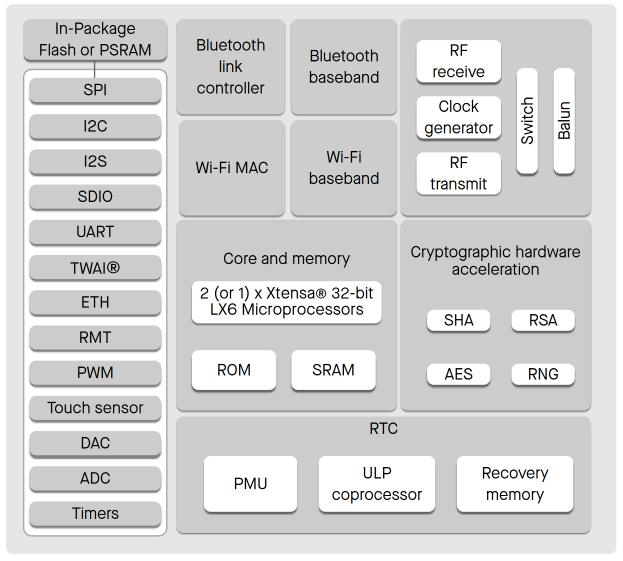
\includegraphics[scale=.5]{abbildungen/functional-block-diagram}
	\caption{ESP32 Functional Block Diagram}
	\label{Fig:esp32-crypto}
\end{figure}

ESP32 chips are equipped with either a single or dual-core Xtensa® 32-bit LX6 microprocessor(s) with up to 240 MHz, 448 KB ROM for booting and core functions, 520 KB SRAM for data and instructions, 34 programmable GPIOs, and cryptographic hardware acceleration. \cite[4-5]{esp32-series}. A functional block diagram of the ESP32 is shown in Figure \ref{Fig:esp32-crypto}. 

The operating system of the ESP32 is freeRTOS \cite[6]{esp32-module}. To develop applications for ESP32, Espressif, the company behind ESP32, provides the ESP-IDF software development framework (ESP-IDF). ESP-IDF provides toolchain, API components and workflows to develop applications for ESP32.
[source programming guide]. Applications and components are written in C 

\begin{figure}
	\centering
	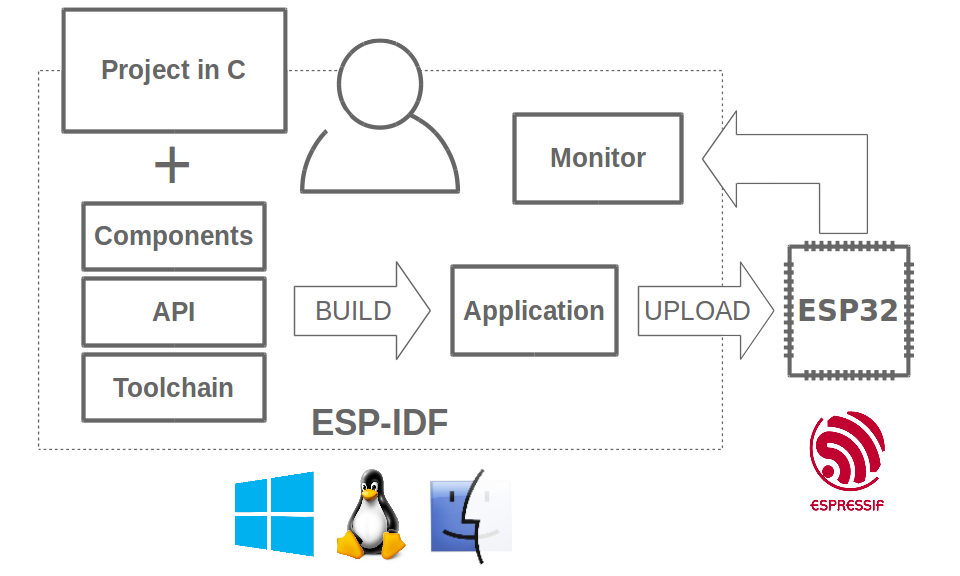
\includegraphics[scale=.5]{abbildungen/esp-idf.png}
	\caption{ESP32 Functional Block Diagram}
	\label{Fig:esp32-crypto}
\end{figure}
[source programming guide]



--development environment


\begin{comment}
    

Build System: CMake
ESP-IDF package manager
Compiler:GCC
\end{comment}